%!TEX root = forallxsol.tex
%\part{Interpretations}
%\label{ch.semantics}
%\addtocontents{toc}{\protect\mbox{}\protect\hrulefill\par}

\setcounter{chapter}{27}
\chapter{Truth in FOL}\setcounter{ProbPart}{0}
\problempart
\label{pr.TorF1}
Consider the following interpretation:
	\begin{ebullet}
		\item The domain comprises only Corwin and Benedict
		\item `$Ax$' is to be true of both Corwin and Benedict
		\item `$Bx$' is to be true of Benedict only
		\item `$Nx$' is to be true of no one
		\item `$c$' is to refer to Corwin
	\end{ebullet}
Determine whether each of the following sentences is true or false in that interpretation:
\begin{earg}
\item $Bc$ \hfill \myanswer{False}
\item $Ac \eiff \enot Nc$ \hfill \myanswer{True}
\item $Nc \eif (Ac \eor Bc)$ \hfill \myanswer{True}
\item $\forall x Ax$ \hfill \myanswer{True}
\item $\forall x \enot Bx$ \hfill \myanswer{False}
\item $\exists x(Ax \eand Bx)$ \hfill \myanswer{True}
\item $\exists x(Ax \eif Nx)$ \hfill \myanswer{False}
\item $\forall x(Nx \eor \enot Nx)$ \hfill \myanswer{True}
\item $\exists x Bx \eif \forall x Ax$ \hfill \myanswer{True}
\end{earg}

\problempart
\label{pr.TorF2}
Consider the following interpretation:	
	\begin{ebullet}
		\item The domain comprises only Lemmy, Courtney and Eddy
		\item `$Gx$' is to be true of Lemmy, Courtney and Eddy.
		\item `$Hx$' is to be true of and only of Courtney
		\item `$Mx$' is to be true of and only of Lemmy and Eddy
		\item `$c$' is to refer to Courtney
		\item `$e$' is to refer to Eddy
	\end{ebullet}
Determine whether each of the following sentences is true or false in that interpretation:
\begin{earg}
\item $Hc$ \hfill \myanswer{True}
\item $He$\hfill \myanswer{False}
\item $Mc \eor Me$ \hfill \myanswer{True}
\item $Gc \eor \enot Gc$ \hfill \myanswer{True}
\item $Mc \eif Gc$ \hfill \myanswer{True}
\item $\exists x Hx$ \hfill \myanswer{True}
\item $\forall x Hx$ \hfill \myanswer{False}
\item $\exists x \enot Mx$ \hfill \myanswer{True}
\item $\exists x(Hx \eand Gx)$ \hfill \myanswer{True}
\item $\exists x(Mx \eand Gx)$ \hfill \myanswer{True}
\item $\forall x(Hx \eor Mx)$ \hfill \myanswer{True}
\item $\exists x Hx \eand \exists x Mx$ \hfill \myanswer{True}
\item $\forall x(Hx \eiff \enot Mx)$ \hfill \myanswer{True}
\item $\exists x Gx \eand \exists x \enot Gx$ \hfill \myanswer{False}
\item $\forall x\exists y(Gx \eand Hy)$ \hfill \myanswer{True}
\end{earg}

\problempart
\label{pr.TorF3}
Following the diagram conventions introduced at the end of \S23, consider the following interpretation:	
\begin{center}
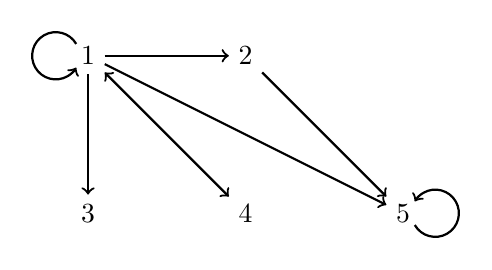
\begin{tikzpicture}
\node (atom1) at (0,2) {1};
\node (atom2) at (2,2) {2};
\node (atom4) at (0,0) {3};
\node (atom5) at (2,0) {4};
\node (atom6) at (4,0) {5};
\draw[->, thick] (atom1)+(-0.15,0.15) arc (-330:-30:.3); 
\draw[->, thick] (atom6)+(0.15,-0.15) arc (-150:150:.3); 
\draw[->, thick] (atom1) -- (atom2);
\draw[->, thick] (atom1) -- (atom4);
\draw[<->, thick] (atom1) -- (atom5);
\draw[->, thick] (atom1) -- (atom6);
\draw[->, thick] (atom2) -- (atom6);
\end{tikzpicture}
\end{center}
Determine whether each of the following sentences is true or false in that interpretation:
\begin{earg}
\item $\exists x Rxx$ \hfill \myanswer{True}
\item $\forall x Rxx$ \hfill \myanswer{False}
\item $\exists x \forall y Rxy$ \hfill \myanswer{True}
\item $\exists x \forall y Ryx$ \hfill \myanswer{False}
\item $\forall x \forall y \forall z ((Rxy \eand Ryz) \eif Rxz)$ \hfill \myanswer{False}
\item $\forall x \forall y \forall z ((Rxy \eand Rxz) \eif Ryz)$ \hfill \myanswer{False}
\item $\exists x \forall y \enot Rxy$ \hfill \myanswer{True}
\item $\forall x(\exists y Rxy \eif \exists y Ryx)$ \hfill \myanswer{True}
\item $\exists x \exists y (\enot x = y \eand Rxy \eand Ryx)$ \hfill \myanswer{True}
\item $\exists x \forall y(Rxy \eiff x = y)$ \hfill \myanswer{True}
\item $\exists x \forall y(Ryx \eiff x = y)$ \hfill \myanswer{False}
\item $\exists x \exists y(\enot x = y \eand Rxy \eand \forall z(Rzx \eiff y = z))$ \hfill \myanswer{True}
\end{earg}

\setcounter{chapter}{29}
\chapter{Using Interpretations}\setcounter{ProbPart}{0}

\solutions
\problempart
\label{pr.Contingent}
Show that each of the following is neither a logical truth nor a contradiction:
\begin{earg}
\item \leftsolutions\ $Da \eand Db$
\item \leftsolutions\ $\exists x Txh$
\item \leftsolutions\ $Pm \eand \enot\forall x Px$
\item $\forall z Jz \eiff \exists y Jy$
\item $\forall x (Wxmn \eor \exists yLxy)$
\item $\exists x (Gx \eif \forall y My)$
\item $\exists x (x = h \eand x = i)$
\end{earg}

\solutions
\problempart
\label{pr.NotEquiv}
Show that the following pairs of sentences are not logically equivalent.
\begin{earg}
\item $Ja$, $Ka$
\item $\exists x Jx$, $Jm$
\item $\forall x Rxx$, $\exists x Rxx$
\item $\exists x Px \eif Qc$, $\exists x (Px \eif Qc)$
\item $\forall x(Px \eif \enot Qx)$, $\exists x(Px \eand \enot Qx)$
\item $\exists x(Px \eand Qx)$, $\exists x(Px \eif Qx)$
\item $\forall x(Px\eif Qx)$, $\forall x(Px \eand Qx)$
\item $\forall x\exists y Rxy$, $\exists x\forall y Rxy$
\item $\forall x\exists y Rxy$, $\forall x\exists y Ryx$
\end{earg}


\problempart
Show that the following sentences are jointly consistent:
\begin{earg}
\item $Ma, \enot Na, Pa, \enot Qa$
\item $Lee, Leg, \enot Lge, \enot Lgg$
\item $\enot (Ma \eand \exists x Ax), Ma \eor Fa, \forall x(Fx \eif Ax)$
\item $Ma \eor Mb, Ma \eif \forall x \enot Mx$
\item $\forall y Gy, \forall x (Gx \eif Hx), \exists y \enot Iy$
\item $\exists x(Bx \eor Ax), \forall x \enot Cx, \forall x\bigl[(Ax \eand Bx) \eif Cx\bigr]$
\item $\exists x Xx, \exists x Yx, \forall x(Xx \eiff \enot Yx)$
\item $\forall x(Px \eor Qx), \exists x\enot(Qx \eand Px)$
\item $\exists z(Nz \eand Ozz), \forall x\forall y(Oxy \eif Oyx)$
\item $\enot \exists x \forall y Rxy, \forall x \exists y Rxy$
\item $\enot Raa$, $\forall x (x=a \eor Rxa)$
\item $\forall x\forall y\forall z[(x=y \eor y=z )\eor x=z]$, $\exists x\exists y\ \enot x= y$
\item $\exists x\exists y((Zx \eand Zy )\eand x=y)$, $\enot Zd$, $d=e$
\end{earg}

\problempart
Show that the following arguments are invalid:
\begin{earg}
\item $\forall x(Ax \eif Bx) \therefore \exists x Bx$
\item $\forall x(Rx \eif Dx), \forall x(Rx \eif Fx) \therefore \exists x(Dx \eand Fx)$
\item $\exists x(Px\eif Qx) \therefore \exists x Px$
\item $Na \eand Nb \eand Nc \therefore \forall x Nx$
\item $Rde, \exists x Rxd \therefore Red$
\item $\exists x(Ex \eand Fx), \exists x Fx \eif \exists x Gx \therefore \exists x(Ex \eand Gx)$
\item $\forall x Oxc, \forall x Ocx \therefore \forall x Oxx$
\item $\exists x(Jx \eand Kx), \exists x \enot Kx, \exists x \enot Jx \therefore \exists x(\enot Jx \eand \enot Kx)$
\item $Lab \eif \forall x Lxb, \exists x Lxb \therefore Lbb$
\item $\forall x(Dx \eif \exists y Tyx) \therefore \exists y \exists z\ \enot y= z$
\end{earg}
